\documentclass[aspectratio=169]{beamer}

\mode<presentation>
%\mode<handout>
{
  \usetheme{Luebeck}
  \usecolortheme{beaver}
  % or ...

  \setbeamercovered{transparent}
  % or whatever (possibly just delete it)
}

\usepackage[english]{babel}
%\usepackage[latin1]{inputenc}
\usepackage{times}
\usepackage[T1]{fontenc}
% \usepackage{natbib}
% \usepackage[natbib=true, bibstyle=authoryear, citestyle=authoryear-comp]{biblatex}
\usepackage{amssymb}
\usepackage{amsmath}
\usepackage{multirow}
\usepackage{graphicx}

\newcommand{\Ivec}[1]{\mbox{\boldmath $#1$}}
\newcommand{\argmin}{\operatornamewithlimits{argmin}}
\newcommand{\argmax}{\operatornamewithlimits{argmax}}
\newcommand{\sgn}{\operatorname{{\mathrm sgn}}}
\newcommand{\mean}{\operatornamewithlimits{mean}}
\newcommand{\Bin}{\operatorname{{\mathrm Bin}}}
\newcommand{\Beta}{\operatorname{{\mathrm Beta}}}
\newcommand{\Gammadist}{\operatorname{{\mathrm Gamma}}}
\newcommand{\Uniform}{\operatorname{{\mathrm Uniform}}}

\beamertemplatenavigationsymbolsempty

% Or whatever. Note that the encoding and the font should match. If T1
% does not look nice, try deleting the line with the fontenc.

\title[How Do We Test Our Hypotheses? A Bayesian Approach] % short title, optional.
{How Do We Test Our Hypotheses?\\A Bayesian Approach}

%%% \subtitle
%%% {Include Only If Paper Has a Subtitle}

\author[Emanuele Olivetti]
{Emanuele Olivetti}

\institute[FBK/CIMeC]
{
  %\inst{1}
  NeuroInformatics Laboratory (NILab)\\
  Fondazione Bruno Kessler, Trento (FBK), Italy\\
  Center for Mind and Brain Sciences (CIMeC),
  University of Trento, Italy\\
  \url{http://nilab.fbk.eu}\\
  \url{olivetti@fbk.eu}}


\date[OHBM2020] % (optional, should be abbreviation of conference name)
{\small Educational Course: Machine Learning for NeuroImaging (ML4NI)}

\subject{}
% This is only inserted into the PDF information catalog. Can be left
% out. 



% If you have a file called "university-logo-filename.xxx", where xxx
% is a graphic format that can be processed by latex or pdflatex,
% resp., then you can add a logo as follows:

%% \pgfdeclareimage[height=1.0cm]{fbk-logo}{figs/Logo-fbk}
%% \logo{\pgfuseimage{fbk-logo}}
%% \pgfdeclareimage[height=1.0cm]{unitn-alfa-logo}{figs/Logo-unitn-alfa}
%% \logo{\pgfuseimage{unitn-alfa-logo}}


% Delete this, if you do not want the table of contents to pop up at
% the beginning of each subsection:


\AtBeginSection[]
{
  \begin{frame}<beamer>{Outline}
    \tableofcontents[currentsection,currentsubsection]
  \end{frame}
}

% \AtBeginSubsection[]
% {
%   \begin{frame}<beamer>{Outline}
%     \tableofcontents[currentsection,currentsubsection]
%   \end{frame}
% }


% If you wish to uncover everything in a step-wise fashion, uncomment
% the following command: 

% \beamerdefaultoverlayspecification{<+->}


\begin{document}

\begin{frame}
  \titlepage
\end{frame}


\begin{frame}
  \begin{center}
    \includegraphics[width=11.5cm]{Fisher_Neyman_Pearson_Jeffreys}
  \end{center}
\end{frame}


\begin{frame}{Ronald Aylmer Fisher (1890-1962)}
  \begin{center}
    \includegraphics[width=5.5cm]{{{R._A._Fischer}}}
  \end{center}
\end{frame}



\begin{frame}{R.A. Fisher: Significance Testing~\cite{fisher1955statistical}}
  \emph{Inductive inference}: from sample to population.
    \begin{block}{The Fisher's recipe}
    \begin{enumerate}
    \item Set up $H_0$, the \emph{null hypothesis} to be disproved with
      the experiment.
    \item Choose a way to summarize of the data into a number, the \emph{test
        statistic} $T$.
    \item Derive the \emph{null distribution} $p(T;H_0)$
      \begin{itemize}
      \item Analytically.
      \item By resampling.
      \end{itemize}
    \item Execute the experiment, collect the data and compute the
      actual value ($T_{obs}$).
    \item Report the $p\text{-value} = p(T \geq T_{obs} ; H_0)$ as a
      measure of evidence against $H_0$.
    \end{enumerate}
  \end{block}
\end{frame}


\begin{frame}{R.A.Fisher: example}
  \begin{columns}
    \small
    \begin{column}{0.6\linewidth}
      \begin{enumerate}
      \item \textbf{Null Hypothesis} $H_0$:\emph{``the classifier predicts at chance level''}
      \item \textbf{Test Statistic} $T$ = \emph{the number of correct predictions} $c$
        (test set size: $n=40$).
      \item \textbf{Null Distribution} $p(c; n=40, p=\frac{1}{2}) =$\\
        $= \Bin(c; n=40, p=\frac{1}{2})$ % = \binom{n}{c} p^c (1-p)^{n-c}$
      \item \textbf{Experiment result:} $c_{obs} = \mathbf{28}$.
      \item $p\text{-value} = p(T \geq 28 ; n=40, p=\frac{1}{2}) =$\\
        $= \sum_{t=28}^{40}\Bin(T=t; n=40, p=\frac{1}{2}) = \mathbf{0.008}$
      \end{enumerate}
    \end{column}
    \begin{column}{0.6\linewidth}
      \includegraphics[width=7.0cm]{binomial_pmf_c28_n40}
    \end{column}
  \end{columns}
\end{frame}


\begin{frame}{Fisher: interpretation of the $p$-value}
  \textbf{Interpretation}:
  \begin{itemize}
  \item A low $p$-value means that $H_0$ may not be a good model.
  \item If $H_0$ is rejected, nothing is said about \emph{what should
      be accepted}.
  % \item \alert{Warning}: The same $p$-value in different experiments
  %   has different meanings.
  \end{itemize}
  \begin{block}{Fisher R.A., Statistical Methods for Research Workers, 1958}
    \emph{``\textbf{Personally}, the writer prefers to set a low standard of
      significance at the 5 percent point...''}
      % A scientific fact should
      % be regarded as \textbf{experimentally established} only if a properly
      % designed
      % experiment rarely fails to give this level of significance.''}
  \end{block}
  % \textbf{\emph{Some} Fallacies}~\cite{goodman2008dirty,hubbard2003confusion}:
  % \begin{enumerate}
  % \item $p\text{-value} = p(T \geq T_{obs};H_0) \text{ }
  %   \alert{\boldsymbol{\neq}} \text{ } p(H_0|\text{data})$
  % \item Replication fallacy: ($1 - p$-value) is \textbf{not} the
  %   probability to replicate a significant result in a repetition of
  %   the experiment.
  % \end{enumerate}
\end{frame}


\begin{frame}{Jerzy Neyman(1894-1981), Egon Pearson(1895-1980)}
  \begin{columns}
    \begin{column}{0.5\linewidth}
      \includegraphics[width=5cm]{0692_03}
    \end{column}
    \begin{column}{0.5\linewidth}
      \includegraphics[width=5cm]{Pearson_Egon_2}
    \end{column}
  \end{columns}
\end{frame}


\begin{frame}{J.Neyman-E.Pearson: Hypothesis Testing}
  \emph{Inductive behaviour}: adjusting behaviour under limited
  information % \cite{neyman1933problem,lehmann2005testing}.
  \begin{block}{Neyman-Pearson recipe}
    \begin{enumerate}
    \item Set up \textbf{two} % SIMPLE
      \emph{complementary} hypotheses: $H_0$
      (\emph{null}) and $H_1$ (\emph{alternative}).
    \item Choose a way to summarize of the data into a number, the
      \emph{test statistic} $T$.
    \item Derive/obtain $p(T;H_0)$ and $p(T;H_1)$ % ~\footnote{Usually adding some
      % assumptions.}
    \item Decide $\alpha = p(\text{reject } H_0; H_0 \text{
        true})$. Decide $n$ (sample size). Compute
      $\beta = p(\text{reject } H_1; H_1 \text{ true})$.
      % \begin{itemize}
      % \item If satisfied go to the next step, otherwise change
      %   $\alpha$, $n$ or $T$ and go back to step 2.
      % \end{itemize}
    \item Compute the for \emph{rejection region}(s) $\mathcal{R}$ for $T$.
    \item Run the experiment and compute the observed $T_{obs}$.
    \item Reject $H_0$ and accept $H_1$ if $T_{obs} \in
      \mathcal{R}$. Or viceversa.
    \end{enumerate}
  \end{block}
\end{frame}


\begin{frame}{J.Neyman-E.Pearson: example}
  \begin{enumerate}
  \item $H_0$:\emph{``the classifier predicts at \textbf{chance level}''}\\
    % $H_1$: :\emph{``the classifier predicts \textbf{better} than
    % chance level''}
    $H_1$: :\emph{``the classifier predicts \textbf{better} than
      chance level.''}
  \item $T$ = \emph{the number of correct predictions} $c$.
  \item $H_0$: $\Bin(c; n=40, \mathbf{p=\frac{1}{2}})$ \\
    $H_1$: $\Bin(c; n=40, \mathbf{p_{MLE}=0.7})$
        \item
          \begin{tabular}{c | c | c}
              $\alpha$ & $\beta$ & $\mathcal{R}_{c\geq}$ \\
              \hline
              % 0.318 & 0.070 & 22 \\
              0.215 & 0.032 & 23 \\
              0.134 & 0.063 & 24 \\
              0.077 & 0.115 & 25 \\
              \textbf{0.040} & \textbf{0.193} & \textbf{26} \\
              0.019 & 0.297 & 27 \\
              % 0.008 & 0.686 & 28 
            \end{tabular}
  \item Rejection region $\mathcal{R} = \{c\geq 26\}$.
  \item Experiment: $c_{obs}=28$.
  \item Report: $H_0$ \textbf{rejected} ($\alpha=0.04$,
    $\beta=0.193$, power=$0.807$).
  \end{enumerate}
\end{frame}


\begin{frame}
  \includegraphics[width=10cm]{{{np_alpha_beta_p0.65_R26}}}
\end{frame}


\begin{frame}{The Anonymous Hybrid ($\sim$1950-)}
  \begin{center}
    \includegraphics[width=5.5cm]{{{Frankenstein's_monster_(Boris_Karloff)}}}
  \end{center}
\end{frame}

\begin{frame}{The \emph{anonymous} hybrid: Fisher + Neyman-Pearson}
  \begin{block}{Anonymous Hybrid's recipe}
    \begin{enumerate}
    \item Set up the null hypothesis $H_0$, choose $T$ and get $p(T;H_0)$.
    \item Choose a threshold $\alpha = p(\text{reject } H_0; H_0 \text{
        true})$, typically $\alpha = 0.05$
    \item Run the experiment and compute the $p$-value under $H_0$.
    \item If $p\text{-value} \leq \alpha$, then:
      \begin{itemize}
      \item \textbf{Reject} $H_0$ and \textbf{accept} $\bar{H_0}$.
      \item Report the result as significant with $p\text{-value} \leq \alpha$
      \end{itemize}
    \end{enumerate}
  \end{block}
  Issues~\cite{goodman2008dirty}:
  \begin{itemize}
  % \item All the issues of the interpretation of the $p$-value.
  \item $\alpha$ without $\beta$ tells very little. % (PPV!).
  \item What is $\bar{H_0}$?
    \begin{itemize}
    \item $p \neq \frac{1}{2}$ ?
    \item The binomial model is not correct?
    \end{itemize}
  \end{itemize}
\end{frame}


\begin{frame}{The \emph{anonymous} hybrid: Fisher + Neyman-Pearson}
  If you like to read more about this topic:
  \begin{itemize}
  \item \cite{gill1999insignificance}
  \item \cite{gigerenzer2004mindless}
  \item \cite{gigerenzer2004null}
  \item \cite{goodman1999toward1,goodman1999toward2}
  \item \cite{hubbard2003confusion}
  \item \cite{berger1987testing}
  \item \cite{sellke2001calibration}
  \item \cite{goodman2008dirty}
  \end{itemize}
\end{frame}


\begin{frame}{Bayesian Hypothesis Testing}
  \begin{center}
    \includegraphics[width=5cm]{{{Harold_Jeffreys,_Sir}}}
  \end{center}
  \begin{center}
    Harold Jeffreys (1891 - 1989)
  \end{center}
\end{frame}

\begin{frame}{Bayesian Concepts}
  \begin{itemize}
  \item $p(X)$ = my degree of belief/knowledge in $X$.
  \item Everything is a random variable, including distribution's
    parameters and hypotheses.
  \item Prior probabilities must be defined.
  \item The Bayesian approach provides a belief calculus.
  \end{itemize}
\end{frame}

\begin{frame}{H.Jeffreys: Bayesian Hypothesis Testing}
  \begin{block}{Bayesian
      recipe~\cite{jeffreys1961theory,kass1995bayes}}
    \begin{enumerate}
    \item Set up \emph{two (or more)} mutually exclusive hypotheses: $H_1$
      and $H_2$.
    \item Quantify \emph{prior probabilities} $p(H_1)$ and $p(H_2)$ from
      current knowledge.
    \item Model the \emph{likelihood of the data}: % (evidence):
      $p(\text{data}|H_1)$, $p(\text{data}|H_2)$.
    \item Run the experiment and collect data.
    \item Compute the \emph{posterior probability} % (analytically or via
      % Monte Carlo)
      \begin{equation*}
        p(H_i|\text{data}) = \frac{p(\text{data}|H_i)
          p(H_i)}{p(\text{data}|H_1) p(H_1) + p(\text{data}|H_2) p(H_2)}
      \end{equation*}
    \item Report the posterior probabilities (or Bayes Factor).
    \end{enumerate}
  \end{block}
\end{frame}

\begin{frame}{H.Jeffreys: example}
  \begin{enumerate}
  \item Hypotheses:
    \begin{itemize}
    \item $H_1$: \emph{``the classifier predicts at chance level''}
    \item $H_2$: \emph{``the classifier predicts better than chance
        level''}
    \end{itemize}
  \item Prior: $p(H_1) = 0.5$, $p(H_2) = 0.5$
  \item Data Likelihoods:
    \begin{itemize}
    % \item $H_1$: $c \sim \Bin(n=40,p=0.5)$
    % \item $H_2$: $c \sim \Bin(n=40, p=\pi)$\\
    %   \quad \enskip $\pi \sim \Uniform(0.5,1)$
    \item $H_1$: $p(c) = \Bin(c | n=40, p=0.5)$
    \item $H_2$: $p(c) = \Bin(c | n=40, p=\pi)$\\
      \quad \enskip $p(\pi) = \Uniform(\pi | 0.5, 1)$      
    \end{itemize}
  \item Run experiment and get the data: $c_{obs}=28$
  \item Posteriors: 
    % \begin{itemize}
    % \item $p(\text{data}|H_1) = \Bin(c=28|n=40,p=0.5) = 0.005$
    % \item $p(\text{data}|H_2) = \text{...[Monte Carlo]...} = 0.097$
    % \end{itemize}
    \begin{itemize}
    \item $p(H_1|\text{data}) = 0.049$
    \item $p(H_2|\text{data}) = 0.951$
    \end{itemize}
    % \begin{itemize}
    % \item $p(H_1|\text{data}) = \frac{p(\text{data}|H_1)
    %     p(H_1)}{p(\text{data}|H_1) p(H_1) + p(\text{data}|H_2) p(H_2)} =
    %   0.049$
    % \item $p(H_2|\text{data}) = \frac{p(\text{data}|H_2)
    %     p(H_2)}{p(\text{data}|H_1) p(H_1) + p(\text{data}|H_2) p(H_2)} =
    %   0.951$
    % \end{itemize}
  \end{enumerate}
  \textbf{Bayes Factor}: $BF_{21} = \frac{p(\text{data}|H_2)}{p(\text{data}|H_1)} = 19.14$
\end{frame}

\begin{frame}{How to compute the posterior probabilities?}
  \begin{itemize}
  \item Prior: $p(H_1) = 0.5$, $p(H_2) = 0.5$
  \item Compute the data likelihood:
    \begin{itemize}
    \item $p(\text{data}|H_1) = \Bin(c=28|n=40,p=0.5) = 0.005$
    \item $\begin{aligned}
      p(\text{data}|H_2) & = \int \Bin(c|n=40, p=\pi)
      \Uniform(\pi|0.5,1) d\pi = \\
      & = \text{...[Monte Carlo]...} = 0.097
      \end{aligned}$
    \end{itemize}
  \item Compute the posteriors:
    \begin{itemize}
    \item $p(H_1|\text{data}) = \frac{p(\text{data}|H_1)
        p(H_1)}{p(\text{data}|H_1) p(H_1) + p(\text{data}|H_2) p(H_2)} =
      0.049$
    \item $p(H_2|\text{data}) = \frac{p(\text{data}|H_2)
        p(H_2)}{p(\text{data}|H_1) p(H_1) + p(\text{data}|H_2) p(H_2)} =
      0.951$
    \end{itemize} 
  \end{itemize}
\end{frame}


\begin{frame}{How to Interpret the Bayes Factor?}
From \cite{jeffreys1961theory,kass1995bayes}
\begin{center}
  \begin{tabular}{c || c }
    $\mathbf{\text{BF}_{2 1}}$ & \textbf{Evidence} \\
    \hline
    \hline
    $< 1$ & Negative (supports $H_1)$\\
    \hline
    $1$ to $3$ & Bare Mention \\
    \hline
    $3$ to $10$ & Substantial \\
    \hline
    $10$ to $30$ & Strong \\
    \hline
    $30$ to $100$ & Very Strong \\
    \hline
    $>100$ & Decisive \\ 
    \hline
  \end{tabular}
\end{center}
\end{frame}

\begin{frame}{Take-home message}
  \begin{itemize}
  \item There is more than one way to test hypotheses.
  \item Learning about the different frameworks is very
    interesting:~\cite{christensen2005testing,berger2003could}.
  \item Which hypothesis framework then?
    \begin{itemize}
    \item Long debate...
    % \item Prof.James Berger: \emph{``use all of them''.}
    \item My opinion: use Bayesian.
    \end{itemize}
  \end{itemize}
\end{frame}




\begin{frame}{Experiments: ICANN2011 MEG competition}
  Tu \& Sun
\begin{columns}
  \begin{column}{0.7\linewidth}
      \begin{tabular}{l|l|c|c|c|c|c|c}
        \multicolumn{2}{c}{}&\multicolumn{5}{c}{Predicted}&\\
        \cline{3-7}
        \multicolumn{2}{c|}{}&\textbf{Art.}&\textbf{Nat.}&\textbf{Foo.}&\textbf{Bean}&\textbf{Cha.}&\multicolumn{1}{c}{}\\
        \cline{2-7}
        \multirow{5}{*}{True}& \textbf{Art.} & 56&   55&   36&    3&    0& 150\\
        \cline{2-7}
        & \textbf{Nat.} & 30&   96&   21&    4&    0& 151\\
        \cline{2-7}
        & \textbf{Foo.} & 33&   22&   46&    1&    0& 102\\
        \cline{2-7}
        & \textbf{Bean} &  4&    3&    3&   95&   20& 125\\
        \cline{2-7}
        & \textbf{Cha.} &  1&    0&    0&   11&  113& 125\\
        \cline{2-7}
        \multicolumn{1}{c}{} & \multicolumn{1}{c}{} & \multicolumn{1}{c}{$124$} & \multicolumn{1}{c}{$176$} & \multicolumn{1}{c}{$106$} & \multicolumn{1}{c}{$114$} & \multicolumn{1}{c}{$123$} & \multicolumn{1}{c}{}\\
      \end{tabular}          
  \end{column}
  \begin{column}{0.32\linewidth}
%      \includegraphics[width=4cm]{tu_and_sun}
  \end{column}
\end{columns}
% \begin{enumerate}
% \item \alert{$p(\{\{1\}, \{2\}, \{3\}, \{4\}, \{5\}\} | \mathbf{N}) = 0.735$}
% \item \alert{$p(\{\{1, 3\}, \{2\}, \{4\}, \{5\}\} | \mathbf{N}) = 0.264$}
% \item $p(\{\{1, 2\}, \{3\}, \{4\}, \{5\}\} | \mathbf{N}) = 0.001$
% \item $p(\{\{1, 2, 3\}, \{4\}, \{5\}\} | \mathbf{N}) \approx 10^{-10}$
% %\item $p(\{\{1\}, \{2, 3\}, \{4\}, \{5\}\} | \mathbf{N}) \approx
% %10^{-10}$
% \setcounter{enumi}{12}
% \item $p(\{\{1, 2, 3\}, \{4, 5\}\} | \mathbf{N}) \approx 10^{-40}$
%   (short vs. long movies)\\
% ... (52 hypotheses) ...
% \end{enumerate}
\end{frame}


\begin{frame}{Experiments: ICANN2011 MEG competition}
  Tu \& Sun
\begin{enumerate}
\item \alert{$p(\{\{Art.\}, \{Nat.\}, \{Foo.\}, \{Bean\}, \{Cha.\}\} | \mathbf{N}) = 0.735$}
\item \alert{$p(\{\{Art., Foo.\}, \{Nat.\}, \{Bean\}, \{Cha.\}\} | \mathbf{N}) = 0.264$}
\item $p(\{\{Art., Nat.\}, \{Foo.\}, \{Bean\}, \{Cha.\}\} | \mathbf{N}) = 0.001$
\item $p(\{\{Art., Nat., Foo.\}, \{Bean\}, \{Cha.\}\} | \mathbf{N}) \approx 10^{-10}$
%\item $p(\{\{Art.\}, \{Nat., Foo.\}, \{Bean\}, \{Cha.\}\} | \mathbf{N}) \approx
%10^{-10}$
\setcounter{enumi}{12}
\item $p(\{\{Art., Nat., Foo.\}, \{Bean, Cha.\}\} | \mathbf{N}) \approx 10^{-40}$
  % (short vs. long movies)\\
\\... (52 hypotheses) ...
\end{enumerate}
\cite{olivetti2012testing,olivetti2020multiclass}
\end{frame}


% % RESULTS FOR ICANN2011: slides_prni2012.py , team Tu & Sun
% % X:
% % [[ 56  55  36   3   0]
% %  [ 30  96  21   4   0]
% %  [ 33  22  46   1   0]
% %  [  4   3   3  95  20]
% %  [  1   0   0  11 113]]
% % alpha:
% % [[ 1.  1.  1.  1.  1.]
% %  [ 1.  1.  1.  1.  1.]
% %  [ 1.  1.  1.  1.  1.]
% %  [ 1.  1.  1.  1.  1.]
% %  [ 1.  1.  1.  1.  1.]]

% % 1) p([[0], [1], [2], [3], [4]] | X) = 0.735500738822
% % 2) p([[0, 2], [1], [3], [4]] | X) = 0.263748106264
% % 3) p([[0, 1], [2], [3], [4]] | X) = 0.000751153684545
% % 4) p([[0, 1, 2], [3], [4]] | X) = 6.49865927897e-10
% % 5) p([[0], [1, 2], [3], [4]] | X) = 5.78964892276e-10
% % 13) p([[0, 1, 2], [3, 4]] | X) = 1.14656906274e-40

% % \begin{frame}
% %   \begin{figure}[h]
% %  \centering
% % \footnotesize{
% % $$\bordermatrix{ \mathbf{I.}&   1&   2&   3&   4&   5\cr
% %   1&   94&  29&  16&  10&   1\cr
% %   2&   22& 100&  10&  18&   1\cr
% %   3&   25&  16&  51&  10&   0\cr
% %   4&   3&   4&  12&  85&  21\cr
% %   5&   2&   2&   4&   3& 114}\quad\quad\quad
% % \bordermatrix{ \mathbf{II.}&   1&   2&   3&   4&   5\cr
% %   1&   56&   55&   36&    3&    0\cr
% %   2&   30&   96&   21&    4&    0\cr
% %   3&   33&   22&   46&    1&    0\cr
% %   4&    4&    3&    3&   95&   20\cr
% %   5&    1&    0&    0&   11&  113}$$
% % }
% % \resizebox{0.7\columnwidth}{!}{%
% %   \begin{tabular}{ c | c | c || c | c |} 
% %     %& & \multicolumn{4}{c}{\textbf{Y}}\\ 
% %     Team & Bin. Test & $B_{10}$ & $B_{1a}$ & $B_{1b}$ \\
% %     \hline
% %     \hline
% %     I & $10^{-156}$ & $10^{169}$ & $10^{67}$ & $10^{11}$\\
% %     \cline{2-5}
% %     II & $10^{-122}$ & $10^{181}$ & $10^{39}$ & \textbf{2.73}\\
% %     \cline{2-5}
% %   \end{tabular}
% % }

% % % 1.60727912872e+181 [array([0, 1, 2, 3, 4])]
% % % 6.50517181267e+39 [array([0, 1, 2]), array([3, 4])]
% % % 1091612047.01 [array([0, 1, 2]), array([3]), array([4])]
% % % 2.72569990995 [array([0, 2]), array([1]), array([3]), array([4])]
% % % 1.32e-122

% % % 7.86540129582e+169 [array([0, 1, 2, 3, 4])]
% % % 4.48036114333e+67 [array([0, 1, 2]), array([3, 4])]
% % % 1.64098820599e+33 [array([0, 1, 2]), array([3]), array([4])]
% % % 110188423978.0 [array([0, 2]), array([1]), array([3]), array([4])]
% % % 6.93e-156

% % \caption{$p$-values and Bayes factors obtained for the confusion
% %   matrices from two of the teams from the ICANN 2011 MEG
% %   competition. \textbf{I}: team Huttunen; \textbf{II}: team Tu \&
% %   Sun. Predictions on the columns and true values on the rows.}
% % \label{fig:meg_results}
% % \end{figure}

% % \end{frame}


\small
\bibliographystyle{apalike}
% \bibliographystyle{plainnat}  

\bibliography{olivetti_tutorial}


\end{document}
